\section{Problem Description}

To achieve this goal, we propose a compartive study that allows to determine the most recommendable technique for extensive DNA sequences, all the way to WGA. We must consider that the latter are usually made up of 5 Giga-base-pairs (Gbp).

\medskip

In Torreno's work \cite{Tirado2015BreakingTC} we observed how a single insertion or deletion of a nucleotide (or character from the previously mentioned alphabet) can cause the rupture of a HSP or aligned fragment. The result was a series of fragments of reduced size, separated by small unaligned substrings. This could have been avoided by using techniques which consider gaps, since those can consider a bound to ignore the \textit{indels}.

\medskip

This idea is further elaborated on Figure \ref{fragmentImprovement}, which illustrates the use of \textit{gaps} as a tool to extend HSPs into larger fragments. In the picture we can observe two graphics which represent the same comparison between two hypothetical sequences: $A$ and $B$. The bottom left alignment is a gapless one, and as such identifies HSPs (of the form $H_i$) of reduced size. 

\medskip

In contrast, the bottom right comparison takes into consideration gaps (of the form $e_i$), which, when added to the HSPs, result in fragments larger in size and closer to each other. 

\begin{figure}
  \centering
  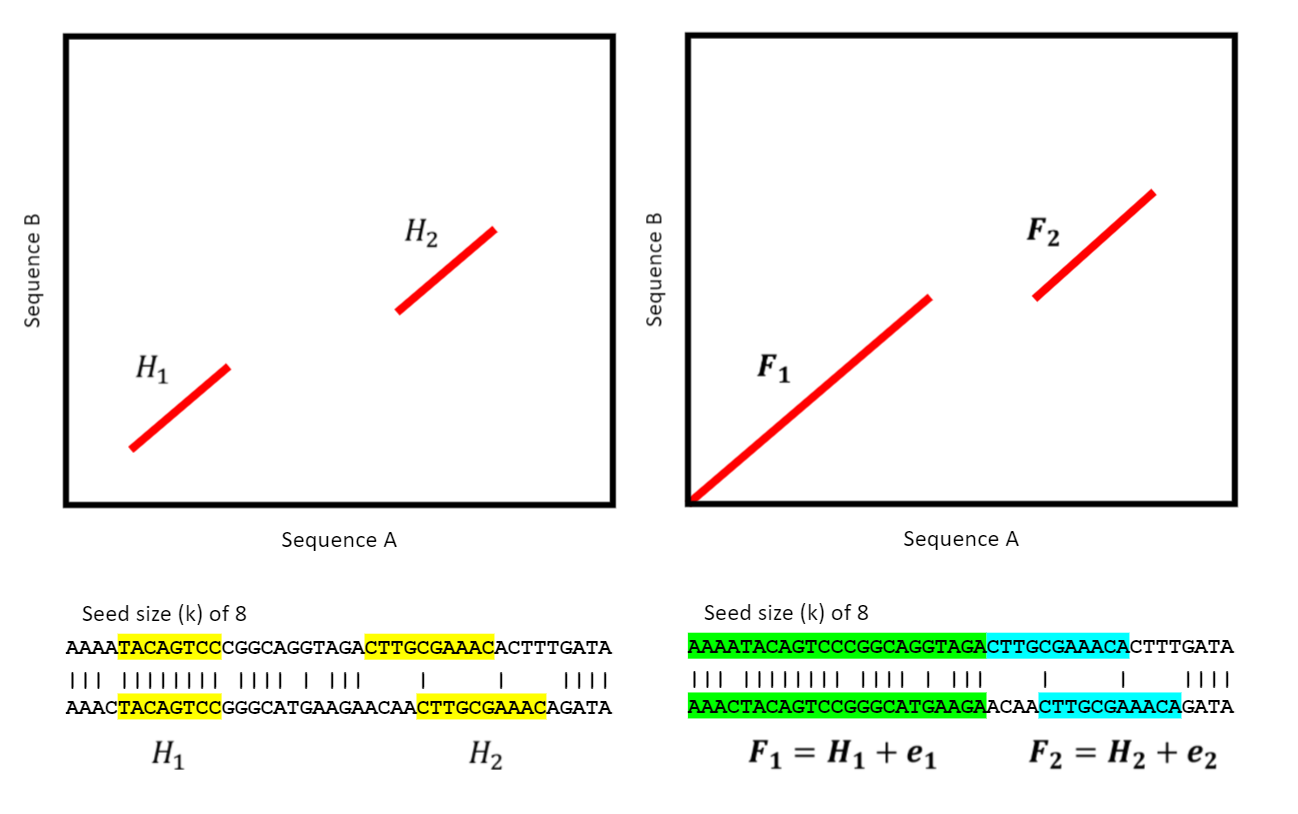
\includegraphics[width=0.95\textwidth]{images/fragmentImprovement.png}
  \caption[]{Example of how the inclusion of \textit{gaps} can result in a better global alignment. Represented as $e_i$, they allow us to obtain larger alignments with variations on only one or two characters.}
  \label{fragmentImprovement}
\end{figure}

\medskip

However, at the moment of writing this document, it is unknown if the results of an alignment that occupies \textit{gaps} are just as valid as the set of alignments without them, as they both cover similar areas of a genomic sequence. 

\medskip

As mentioned before, the use of \textit{gaps} may represent an issue since they increase the spatial requirements for the alignment to be performed. This is due to the parameters required for the comparison, the spaces generated in the fragments that are being compared, and the penalization given to each individual gap. However, as mentioned, their inclusion can transform a set of various HSPs of reduced size into a considerably better aligned one. 

\medskip

Despite their consideration as a useful tool for sequence alignments, to our knowledge there is no consensus over the cases of use in which employing \textit{gaps} should be the norm, as well as the penalization that should be assigned to them.

\medskip

Based on the researched literature, and the possibility of a contribution to this dilemma, we state the following research problem:

\begin{quote}
  ``The lack of a consensus regarding the higher sensibility and specifity, in exchange for higher computational requirements in intergenomic alignments with and without the use of \textit{gaps}."
\end{quote}